\documentclass[12pt, a4paper]{report}
\usepackage[utf8]{inputenc}
\usepackage[T1]{fontenc}
\usepackage[utf8]{inputenc}
\usepackage{geometry}
\usepackage{listings}
\usepackage{xcolor}
\usepackage[]{graphicx}

\definecolor{codegreen}{rgb}{0.26, 0.61, 0}
\definecolor{codegray}{rgb}{0.5,0.5,5}
\definecolor{codepurple}{rgb}{58,0,0.82}
\definecolor{backcolour}{rgb}{0.80, 0.81, 0.93}

\lstdefinestyle{mystyle}{
    backgroundcolor=\color{backcolour},   
    commentstyle=\color{codegreen},
    keywordstyle=\color{magenta},
    numberstyle=\tiny\color{codegray},
    stringstyle=\color{codepurple},
    basicstyle=\ttfamily\footnotesize,
    breakatwhitespace=false,         
    breaklines=true,                 
    captionpos=b,                    
    keepspaces=true,                 
    numbers=left,                    
    numbersep=5pt,                  
    showspaces=false,                
    showstringspaces=false,
    showtabs=false,                  
    tabsize=2
}

\lstset{style=mystyle}


\title{\textbf{EE2703: Applied Programming Lab\\Assignment 3\\Fitting Data to Models}}


\author{Devaganthan S S\\ EE19B018}
\date{\today}
\begin{document}

\maketitle


\section{Abstract}
Aim of this experiment is to,
\begin{itemize}
    \item Analysing the data to extract information
    \item Study the effect of noise on the fitting process
    \item Learn to plot Graphs in python
\end{itemize}

\section{Introduction}
With the help of computers, it has become very easy to model data. This helps us in predicting things.
In this experiment, we try modelling the data, generated using the {\fontfamily{cmss}\selectfont
'generate\_data.py'
}. With the help of python, we try fitting the data into a function. The function generated is verified by several means.

\section{Implementation}
The data file has to be passed as an argument in the command line, while running the code. The program prints a set of instructions. Based on the requirement, input has to be given

\section{Results}
\subsection{Generating and Loading Data}
Using the {\fontfamily{cmss}\selectfont
'generate\_data.py'
}, a file named {\fontfamily{cmss}\selectfont
'fitting.dat'
} is created, which contains data required for the experiment. The file comprises of 10 columns with 101 rows each. The first column is time. The rest 9 columns are data, with noise, having different standard deviation in the range $10^{-3}$  to $10^{-1}$

\noindent
The data is loaded into the program using the function {\fontfamily{cmss}\selectfont
'loadtxt()'
} 
\subsection{Plotting the Data and True Value}
The columns in the data are plotted against time. Each column corresponds to $f(t)+noise$. The noise is not same for all columns. The below code plots the graph in Python.

\lstinputlisting[language = python]{code1.py}
 \ 
 \break
\noindent
The Output Graph is below,
\begin{figure}[h!]
    \centering
    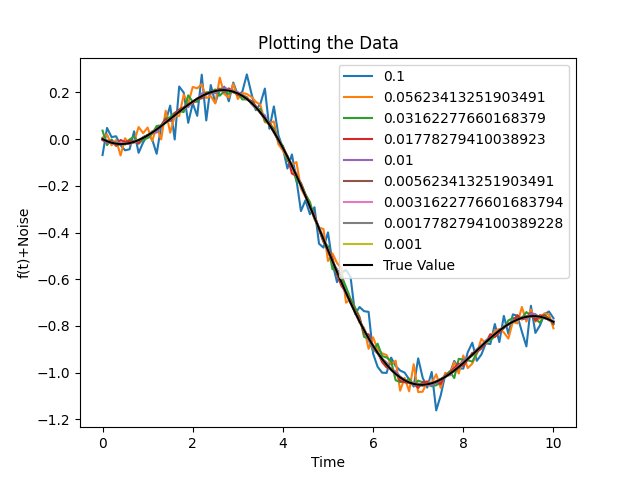
\includegraphics[scale=1]{Figure_1.png} 
    \caption{}
    \label{fig:my_label}
\end{figure}

\subsection{Plotting the Error Bars:}
The error bars are plotted using the function {\fontfamily{cmss}\selectfont
'errorbar()'
}, for every 5th item of the first column. Also, the exact curve is plotted to understand how much the data diverges. The below code accomplishes the above,\
 
\vspace{5mm} %5mm vertical space
\noindent
\lstinputlisting[language = python]{errorbar.py}
 \ 
 \break
\noindent
The Output Graph is below,
\begin{figure}[h]
    \centering
    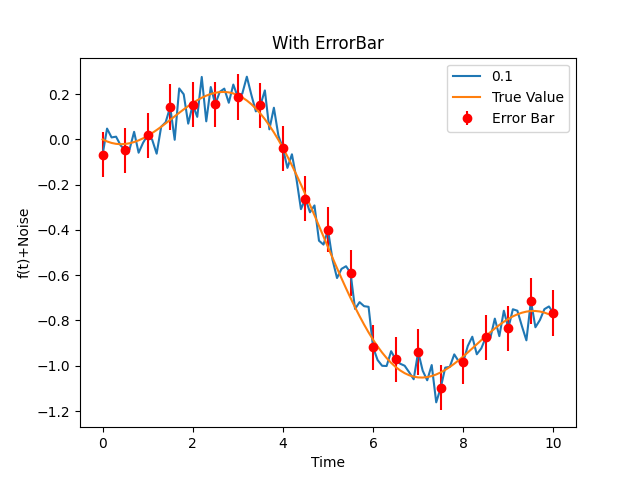
\includegraphics[scale=0.89331799999]{ErrorBar.png} 
    \caption{}
    \label{fig:my_label}
\end{figure}
\subsection{Constructing the Coefficient Matrix:}
The M matrix is generated, with $J(t)$ as its first column and time as its second column. The Vector $M.\left(\begin{array}{cc}
    A_O\\
    B_O 
\end{array}\right)$ is generated using the {\fontfamily{cmss}\selectfont
'dot()'
} function, where $A_O$ is 1.05 and $B_O$ is -0.105. With the $g(t, A, B)$ function, a column vector is generated with $A$ and $B$ as 1.05 and -0.105 where $t$ is the time vector. The two columns generated are equal and they are verified by taking a sum of squared differences, and it turns out to be zero. The below code accomplishes the above tasks.
 
\vspace{5mm} %5mm vertical space
\noindent
\lstinputlisting[language = python]{mMatrixGen.py}

\subsection{Mean Square Error Matrix and Contour Plot}
For $A = 0,0.1,…….,2$ and $B = -0.2,-0.19,…….,0$ for the data given in Column 1, the mean squared error is computed which is given by,
\vspace{5mm}
\begin{equation}\label{eq:4}
\epsilon_{ij}=\frac{1}{101}\sum_{k=0}^{101}\left(f_{k}-g(t;A_i,B_j)\right)^{2}
\end{equation}

 The Mean Squared Error is stored as a Matrix given by ‘E’. With this matrix, a contour plot is generated to analyze errors produced by different values of A and B. The above is accomplished by the below code
\vspace{4mm}
\noindent
\lstinputlisting[language = python]{MSE_contourPlot.py}
 \ 
 \break
\noindent
The Output Graph is below,
\begin{figure}[h!]
    \centering
    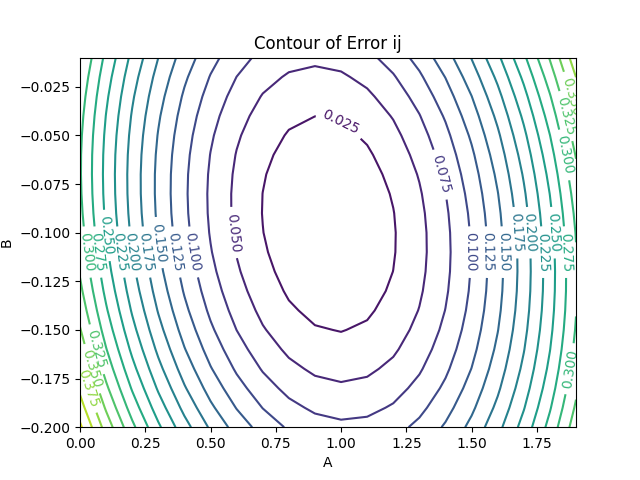
\includegraphics[scale=0.62150]{ContourPlot.png} 
    \caption{}
    \label{fig:my_label}
\end{figure}
\vspace{1mm}


 From the Contour plot, we can see that, there is only 1 minimum. The graph seems to have a minimum near A = 1.05 and B = -0.105.

\subsection{Best Approximate for A and B}
The best approximate for A and B is computed for each data Column using the {\fontfamily{cmss}\selectfont
'lstsq()'
} function from {\fontfamily{cmss}\selectfont
'scipy.linalg'
}. The above is accomplished by the below code.
 
\vspace{5mm} %5mm vertical space
\noindent
\lstinputlisting[language = python]{bestEst.py}

\subsection{Plotting Error in the Estimate}
The error in the estimate of A and B is computed using the mean Square method for data files which has noises of different standard deviations. Then the estimate of A and B are plotted as a function of the standard deviation, $\sigma$. The below code accomplishes the above,
\vspace{5mm}
\noindent
\lstinputlisting[language = python]{errorplot.py}
\vspace{50mm}
The Output Graph is below,
\begin{figure}[h!]
    \centering
    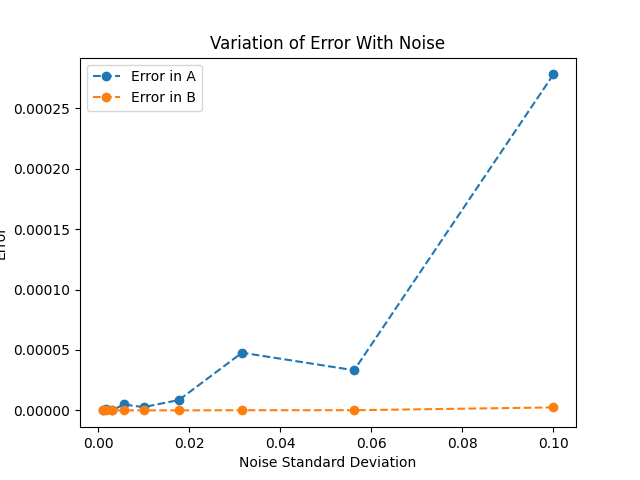
\includegraphics[scale=0.8]{ErrorPLot.png} 
    \caption{}
    \label{fig:my_label}
\end{figure}
\vspace{1mm}

\noindent
From the graph, we can notice that the error seems to increase linearly with the standard deviation.\\

\vspace{2mm}
\noindent
The same plot is redone using {\fontfamily{cmss}\selectfont
'loglog()'
} to display the plot in logscale. The below code accomplishes it,
\vspace{2mm}
\lstinputlisting[language = python]{loglog.py}
The Output Graph is,
\begin{figure}[h!]
    \centering
    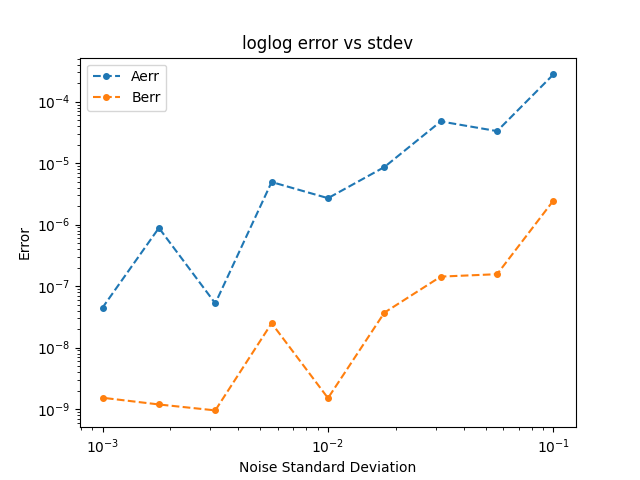
\includegraphics[scale=0.8]{loglog.png} 
    \caption{}
    \label{fig:my_label}
\end{figure}
\vspace{1mm}

\noindent
The error is approximately linear with respect to standard deviation except for a few points.\\
\section{Conclusion:}
From this experiment, I have learned how to plot functions in python. I learnt how to model a given set and compute the error in the Model.
\end{document}

